\documentclass[conference]{IEEEtran}
\IEEEoverridecommandlockouts
\usepackage{cite}
\usepackage{amsmath,amssymb,amsfonts}
\usepackage{algorithmic}
\usepackage{graphicx}
\usepackage{multirow}
\usepackage{url}
\usepackage{tikz}
\usepackage{pgfplots}
\pgfplotsset{compat=1.18}
\pgfplotsset{log ticks with fixed point}
\usetikzlibrary{shapes.geometric, arrows.meta, positioning, fit, backgrounds, calc}
\usepackage{textcomp}
\usepackage{xcolor}
\def\BibTeX{{\rm B\kern-.05em{\sc i\kern-.025em b}\kern-.08em T\kern-.1667em\lower.7ex\hbox{E}\kern-.125emX}}

\begin{document}

\title{Reducing False Alarms in Edge Driver Monitoring Systems via Negative-Frame Curation}

\author{\IEEEauthorblockN{Author names are omitted for double-blind review}
\thanks{This work involved human subjects in its research. The author(s) confirm(s) that all human subject research procedures and protocols are exempt from review board approval. This study reuses publicly available, de-identified data from the Driver Monitoring Dataset (DMD) and did not involve new data collection from human participants.}}

\maketitle

\begin{abstract}
Frequent false alarms in edge-deployed driver monitoring systems degrade driver trust, waste on-device computing cycles, and elevate thermal load. This paper evaluates whether curating negative training frames reduces false alarms and whether replacing randomly sampled negative frames with hard-mined false positives provides further suppression. Four lightweight You Only Look Once (YOLO) object detection models were trained and benchmarked on a 15,723-frame dataset extracted from the Driver Monitoring Dataset across four localized visual cues using a dedicated graphics processing unit. Models were evaluated across negative-frame ratios ranging from 0\% to 80\%, followed by hard-negative mining trials and an edge deployment benchmark measuring runtime overhead. Results demonstrate that increasing negative frames consistently reduces false alarms across all architectures, with hard-negative mining achieving an additional reduction of up to 68\%. Crucially, mean average precision, recall, and target cue sensitivity remain stable while precision increases, confirming that false-alarm suppression does not compromise target detection accuracy. These findings show that negative-frame curation and hard-negative mining serve as effective, model-agnostic techniques to curb nuisance alerts, prevent automation disuse, and reduce computational overhead on in-cabin edge hardware.
\end{abstract} % DONE 

\begin{IEEEkeywords}
Driver monitoring systems, object detection, false alarm suppression, hard-negative mining, edge computing.
\end{IEEEkeywords} % DONE 

\section{Introduction}
Starting in July 2026, European Union (EU) vehicle-safety regulations require advanced driver distraction warning systems in new vehicles \cite{ec2026safercars}. 
Early vision-based Driver Monitoring Systems (DMS) estimated driver states using spatio-temporal action recognition \cite{ortega2020dmd, canas2021detection}. 
However, these three-dimensional convolutional architectures require excessive memory and compute time, making them unsuitable for low-power automotive microcontrollers \cite{canas2021detection, florez2024real}. 
Modern edge DMS pipelines instead formulate monitoring as frame-by-frame object detection \cite{yolodrive2025, pyolov82024}. 
These pipelines deploy lightweight models such as the You Only Look Once (YOLO) detector family to identify localized behavioral cues, including phone use, drinking, and eye closure \cite{ortega2020dmd, yolov12dms2025}. 
In-cabin edge hardware must run these models under strict limits: inference latency must remain under 30\,ms \cite{liu2019edge}, and power draw must stay below 10--15\,W to avoid overheating \cite{florez2024real, benoitcattin2020thermal}. 

Lightweight detectors meet these power and latency targets, but existing DMS datasets consist almost entirely of positive distraction events \cite{yolodrive2025, pyolov82024}. 
Because single-frame detectors lack temporal context, models trained without negative examples generate frequent false positives on benign objects like steering wheel contours, seat belts, and clothing folds \cite{canas2021detection}. 
In real-world driving, normal (non-distracted) conditions account for the vast majority of operating time, empirically estimated in this study's curated corpus at approximately 81\% of frames. 
Frequent false alarms during normal driving cause alert fatigue, leading drivers to ignore, mute, or bypass safety systems entirely \cite{lambert2026chinese, parasuraman1997humans}. 
These false alarms also trigger downstream tasks, including facial landmark tracking, Controller Area Network (CAN) bus logging, and video recording \cite{florez2024real, liu2019edge}. 
These secondary tasks create processing spikes that cause thermal throttling on embedded chips \cite{benoitcattin2020thermal}. 
Adding negative (background-only) frames during training reduces false alarms, but the impact of negative-sampling ratios and hard-negative mining has not been thoroughly evaluated in edge DMS applications \cite{ultralytics2023guidelines, jin2018video}. 

To address these challenges, this paper provides three main contributions: 
\begin{itemize}
    \item \textbf{Negative Sampling Benchmarks:} A systematic evaluation of negative-to-positive frame ratios (0\% to 80\%) across four lightweight edge object detectors (YOLO11n, YOLO26n, YOLO12n, and YOLOv10n) \cite{yolodrowsiness2025, yolov12dms2025}. 
    \item \textbf{Hard-Negative Mining Analysis:} An experimental evaluation showing that targeted hard-negative mining lowers the false alarm rate (FAR) by up to 67.8\% without reducing cue detection accuracy \cite{shrivastava2016ohem}. 
    \item \textbf{Edge Deployment Study:} An operational evaluation projecting nuisance alerts per hour ($\mathcal{A}_h$) across streaming frame rates and validating sub-30\,ms execution on edge hardware \cite{liu2019edge}. 
\end{itemize}

Specifically, this study answers two central research questions (RQs): 
\begin{itemize}
    \item \textbf{RQ1:} What ratio of negative-to-positive training frames minimizes false alarms without reducing cue detection sensitivity, and is this ratio consistent across different lightweight architectures? 
    \item \textbf{RQ2:} Does replacing random negative frames with hard negatives (prior false positives) provide better false-alarm suppression in resource-constrained models? 
\end{itemize}
% DONE 
\section{Related Work}

\subsection{Vision-Based Driver Monitoring and Localized Cue Detection}
Vision-based DMS historically approached driver state estimation as a holistic action recognition task, applying deep convolutional neural networks (CNNs) to classify temporally clipped video segments into coarse behavioral categories such as safe driving, talking, or drinking \cite{ortega2020dmd, canas2021detection}. Comprehensive multi-modal datasets, such as the Driver Monitoring Dataset (DMD) \cite{ortega2020dmd} and Drive\&Act \cite{martin2019drive}, established standardized evaluation benchmarks across red-green-blue (RGB), depth, and infrared camera feeds. However, holistic spatio-temporal architectures, including 3D-CNNs and multi-stage pose long short-term memory (LSTM) networks, incur high computational latency and memory footprints that exceed the processing capabilities of low-cost embedded automotive microcontrollers \cite{canas2021detection, florez2024real}.

To satisfy strict real-time execution constraints, modern edge DMS architectures increasingly formulate driver monitoring as localized object detection, leveraging lightweight single-stage detectors from the YOLO family to identify localized behavioral cues (e.g., handheld phone usage, drinking, and eye closure) on a frame-by-frame basis \cite{yolodrive2025, yolov12dms2025, pyolov82024}. Recent works have proposed specialized architectural modifications; for instance, YOLO-Drive integrates state-space EfficientViM blocks and polarized attention to disentangle overlapping distraction cues \cite{yolodrive2025}, while pruned YOLOv8 and compact YOLOv11 variants optimize bounding-box inference for micro-edge deployment \cite{pyolov82024, yolodrowsiness2025}.

Nonetheless, existing cue detection models are trained almost exclusively on benchmark splits curated from positive distraction intervals \cite{yolodrive2025, pyolov82024}. Because single-stage detectors lack temporal priors, they exhibit frequent background false-positive detections when deployed in unconstrained operational environments, misclassifying steering wheel contours, seat belts, and clothing folds as hazard cues. Existing literature focuses primarily on maximizing mean Average Precision (mAP) on positive-skewed test splits, leaving the problem of background false-alarm suppression in lightweight DMS detectors largely unaddressed.

\subsection{Automotive Edge Computing and Cascading Thermal Overhead}
Sustaining the latency and power bounds introduced in Section~I is challenging under passive cooling: automotive edge platforms must maintain sub-30\,ms inference within power envelopes below 10--15\,W in enclosed cabin electronics bays \cite{florez2024real, liu2019edge}. Prior embedded DMS studies, such as the Jetson Nano framework evaluated by Florez \textit{et al.} \cite{florez2024real}, report isolated frame rates and nominal wattage under static test streams.

However, in an integrated automotive edge pipeline, an object detection trigger initiates a cascade of computationally intensive secondary tasks, including high-precision facial landmark alignment, trajectory tracking, CAN bus event logging, and local ring-buffer video encoding \cite{florez2024real, liu2019edge}. When an unregularized detector generates frequent false positives on benign cabin artifacts, these secondary routines execute continuously. Benoit-Cattin \textit{et al.} demonstrated that sustained processing spikes on edge vision processors rapidly trigger thermal throttling, driving dynamic frequency scaling that can reduce inference throughput by more than 40\% and induce severe latency spikes \cite{benoitcattin2020thermal}. Despite this operational risk, prior DMS literature evaluates detection models in isolation, overlooking how frame-level false-positive rates compound over time into unsustainable hourly nuisance alert rates ($\mathcal{A}_h$) across practical operating frame rates, driving unnecessary edge compute and thermal strain.

\subsection{Alert Fatigue, Automation Disuse, and Regulatory Mandates}
DMS operational reliability is central to the EU Advanced Driver Distraction Warning mandate introduced in Section~I, which requires reliable warning escalation once gaze distraction exceeds specified temporal limits \cite{ec2026safercars}.

However, system safety is severely compromised when models trigger persistent false alarms. Human-automation interaction theory, established by Parasuraman and Riley, shows that false alarms are the primary cause of automation \textit{disuse}, defined as the deliberate ignoring, muting, or disabling of safety systems by human operators \cite{parasuraman1997humans}. In real-world driving, repeated nuisance alerts rapidly induce alert fatigue, eroding driver trust \cite{parasuraman1997humans}. This loss of trust has driven motorists to deploy aftermarket defeat devices, such as mounted mannequin heads that fool cabin monitoring cameras into classifying a non-existent alert face, prompting regulatory vehicle recalls of over 2.7 million vehicles in China \cite{lambert2026chinese}. While regulatory mandates evaluate sensitivity, existing academic DMS literature fails to address false-alarm suppression as a foundational requirement for driver acceptance and regulatory viability.

\subsection{Negative-Frame Curation and Hard-Negative Mining}
To suppress false positives, object detection literature has historically focused on loss-formulation reweighting, such as Focal Loss \cite{lin2017focal} to balance candidate box gradients, or Online Hard Example Mining (OHEM) \cite{shrivastava2016ohem} to backpropagate high-loss proposals in two-stage detectors. However, OHEM is computationally unsuitable for single-stage lightweight YOLO models, and loss reweighting fails when the training set entirely lacks unannotated negative images \cite{lin2017focal}.

At the dataset level, practitioner heuristics commonly suggest adding 0\% to 10\% background images (frames containing no bounding boxes) to regularize the detection head \cite{ultralytics2023guidelines}. Yet, this 0--10\% recommendation is an arbitrary heuristic developed for general object detection benchmarks, lacking empirical validation in automotive environments where benign driving comprises over 95\% of operational time. Moreover, random negative frames offer diminishing returns because unchallenging background scenes generate minimal gradient feedback \cite{shrivastava2016ohem, jin2018video}. While video mining strategies harvest temporal flicker as hard negatives in generic domains \cite{jin2018video}, no prior work has systematically evaluated negative-frame curation ratios (from 0\% to 80\%) across multiple lightweight YOLO architectures, nor measured how hard-negative mining suppresses operational nuisance alert frequencies on edge hardware.% DONE 
\section{Methodology}
This section outlines the experimental methodology designed to address two central research questions:
\begin{itemize}
    \item \textbf{RQ1 (Negative Sampling Ratio):} What ratio of negative-to-positive training frames minimizes background false alarms without degrading localized cue detection sensitivity, and is this threshold consistent across lightweight detector architectures?
    \item \textbf{RQ2 (Hard-Negative Mining):} Does replacing uniformly sampled negative frames with hard negatives (prior false positives) provide superior false-alarm suppression at matched training dataset size?
\end{itemize}
Subsections~\ref{subsec:arch}--\ref{subsec:metrics} define the architectures, dataset curation, split protocols, and evaluation metrics used for RQ1, while Subsections~\ref{subsec:mining}--\ref{subsec:deployment} detail the mining protocol and deployment benchmarks used for RQ2.

\subsection{Model Architectures and Training Configuration}
\label{subsec:arch}
We evaluate four lightweight YOLO detector variants selected for edge deployment due to their compact footprints (fewer than 3~million parameters): YOLO11n, YOLO26n, YOLO12n, and YOLOv10n. Table~\ref{tab:models} summarizes each model's parameter count, computational cost in giga floating-point operations (GFLOPs), and input resolution.

All models are initialized from pretrained Common Objects in Context (COCO) weights using the Ultralytics framework. Training hardware and hyperparameters, including the graphics processing unit (GPU) and video RAM (VRAM), are summarized in Table~\ref{tab:training_config}. Standard data augmentations include mosaic augmentation (disabled for the final 10 epochs via \texttt{close\_mosaic=10}), random horizontal flipping ($p = 0.5$), hue-saturation-value (HSV) color-space adjustments, random translation ($\pm 10\%$), and random erasing ($p = 0.4$). Geometric distortions (rotation, shear, and perspective distortion) are disabled to preserve realistic in-cabin camera geometry. The random-seed protocol used across negative-ratio configurations is detailed in Section~\ref{subsec:splits}.

\begin{table}[htbp]
\caption{Training Hardware and Hyperparameters}
\begin{center}
\begin{tabular}{|l|l|}
\hline
\textbf{Parameter} & \textbf{Value} \\
\hline
GPU                & NVIDIA RTX 4060 (8\,GB VRAM) \\
Pretrained weights & COCO \\
Epochs             & 100 \\
Batch size         & 16 \\
Optimizer          & AdamW \\
Initial LR         & 0.00125 \\
LR schedule        & Linear decay \\
Input size         & $640 \times 640$ \\
\hline
\end{tabular}
\label{tab:training_config}
\end{center}
\end{table}

\begin{table}[htbp]
\caption{Evaluated YOLO Architectures}
\begin{center}
\begin{tabular}{|c|c|c|c|}
\hline
\textbf{Model} & \textbf{Params (M)} & \textbf{GFLOPs} & \textbf{Input Size} \\
\hline
YOLO11n  & 2.6 & 6.5 & $640\times640$ \\
YOLO26n  & 2.6 & 6.2 & $640\times640$ \\
YOLO12n  & 2.6 & 7.6 & $640\times640$ \\
YOLOv10n & 2.3 & 6.6 & $640\times640$ \\
\hline
\end{tabular}
\label{tab:models}
\end{center}
\end{table}

\subsection{Dataset Curation and Annotation Protocol}
Our evaluation uses video streams from the DMD \cite{ortega2020dmd}, covering 14 drivers across both stationary and driving conditions. We sample frames at a rate of 1 frame per second (FPS) from 81 RGB recordings, yielding 15,723 face-crop images at $640 \times 640$ resolution. All sampled frames are retained without post-sampling filtering. The curated set consists of 19\% positive cue frames (3,001 frames) and 81\% negative frames (12,722 frames), reflecting the natural rarity of distraction events in routine driving.

Each image contains either zero or one bounding box. Negative frames contain no bounding boxes, capturing distraction-free baseline driving. Positive frames contain a single localized bounding box identifying one of four behavioral cues: yawning, hand-over-mouth, drinking, or phone use.

A single human annotator completed the annotations in one pass without an independent second annotator for agreement scoring. The annotation protocol enforces three key rules:
\begin{itemize}
    \item \textbf{Mutual Exclusion:} Yawning and hand-over-mouth cannot co-occur. If a driver covers a yawn with their hand, hand-over-mouth takes precedence.
    \item \textbf{Visible Anatomy Only:} Bounding boxes tightly enclose visible target cues. Occluded, truncated, or out-of-frame regions are not estimated, though partially occluded cues remain valid if visually identifiable.
    \item \textbf{Scale Invariance:} No minimum pixel-size cutoff is applied to bounding boxes at the $640 \times 640$ input scale.
\end{itemize}

\subsection{Training Splits, Negative Ratios, and Seed Protocol}
\label{subsec:splits}
We partition the dataset using an 80/10/10 stratified split across the 3,001 positive cue frames. This yields a fixed positive core of 2,401 frames for training, while the validation and test sets each receive 300 positive frames.

To address RQ1, we construct five training configurations by augmenting the 2,401 positive training frames with varying proportions of negative frames, spanning ratios from 0\% to 80\% (Table~\ref{tab:splits}). Both the validation and test sets maintain a fixed 80.9\% negative ratio (1,272 negative and 300 positive frames, 1,572 total each) to mirror automotive driving environments where baseline driving accounts for the vast majority of operational time.

To account for stochastic variation from weight initialization and mini-batch shuffling, configurations with higher sampling variance (0\%, 20\%, and 40\%) are trained across two random seeds ($\text{seed} \in \{42, 43\}$), while 60\% and 80\% configurations are trained across a single seed ($\text{seed}=42$), as summarized in Table~\ref{tab:seeds}. Metrics for two-seed configurations are reported as the mean across seeds.

\begin{table}[htbp]
\caption{Random Seed Protocol by Negative Ratio}
\begin{center}
\begin{tabular}{|c|c|}
\hline
\textbf{Negative Ratio} & \textbf{Seeds Used} \\
\hline
0\%, 20\%, 40\% & 42, 43 \\
60\%, 80\%      & 42 \\
\hline
\end{tabular}
\label{tab:seeds}
\end{center}
\end{table}

\subsection{Evaluation Metrics and False-Alarm Quantification}
\label{subsec:metrics}
We report three categories of metrics: detection accuracy (precision, recall, and F1 score), localization quality (mAP), and operational false alarms (false alarm rate (FAR) and false positives per 1{,}000 frames (FP/1k)).

A predicted bounding box is counted as a True Positive (TP) if it overlaps a ground-truth box by at least $0.50$ Intersection over Union (IoU) and predicts the correct driver-cue class. Otherwise, it is counted as a False Positive (FP). A ground-truth target with no matching prediction is counted as a False Negative (FN). Precision and recall are defined as:
\begin{equation}
\text{Precision} = \frac{\text{TP}}{\text{TP} + \text{FP}}, \quad \text{Recall} = \frac{\text{TP}}{\text{TP} + \text{FN}}.
\label{eq:precision_recall}
\end{equation}

The F1 score summarizes precision and recall at the maximum-$F_1$ operating threshold:
\begin{equation}
F1 = 2 \cdot \frac{\text{Precision} \cdot \text{Recall}}{\text{Precision} + \text{Recall}}.
\label{eq:f1}
\end{equation}

Localization quality is measured via mAP averaged across the four driver-cue categories (yawning, hand-over-mouth, drinking, and phone use). We report $\text{mAP}_{50}$ at a fixed IoU threshold of $0.50$:
\begin{equation}
\text{mAP}_{50} = \frac{1}{C} \sum_{c=1}^{C} \text{AP}_c^{50}, \quad C = 4,
\label{eq:map}
\end{equation}
where $\text{AP}_c^{50}$ denotes the Average Precision (AP) for driver-cue class $c$ at an IoU threshold of $0.50$, and $C$ represents the total number of cue classes. We also report $\text{mAP}_{50:95}$, which averages AP across ten IoU thresholds from $0.50$ to $0.95$ at increments of $0.05$.

To measure operational reliability on frames devoid of safety events, let $\mathcal{D}_{\mathrm{eval}}^{\mathrm{neg}}$ denote the set of $N_{\mathrm{neg}} = 1{,}272$ background-only frames in an evaluation split. Let $FP_{\mathrm{neg}}$ be the total number of detections with confidence at or above threshold $\tau = 0.25$ produced across all frames in $\mathcal{D}_{\mathrm{eval}}^{\mathrm{neg}}$. We define the per-frame FAR and the scaled operational metric FP/1k as:
\begin{equation}
\text{FAR} = \frac{FP_{\mathrm{neg}}}{N_{\mathrm{neg}}}, \qquad \mathrm{FP/1k} = 1000 \times \text{FAR}.
\label{eq:far}
\end{equation}

FAR and FP/1k serve as primary outcome metrics for RQ1 and RQ2. We report precision, recall, F1, and mAP concurrently to verify that background regularization suppresses false alarms without reducing cue detection sensitivity.

\subsection{Hard-Negative Mining Protocol}
\label{subsec:mining}
To address RQ2, we implement the hard-negative curation pipeline illustrated in Fig.~\ref{fig:combined_framework}(b). First, we train a baseline detector $f_{\theta_0}$ using the 0\% negative configuration (Table~\ref{tab:splits}), which contains only positive cue frames. Because this detector is trained without background scenes, it readily produces false positives on non-target cabin textures, making it an effective filter for identifying challenging negative frames.

Next, we run $f_{\theta_0}$ in batched inference over the pool of unselected training negative frames ($\mathcal{U}_{\mathrm{neg}}$, separate from the held-out evaluation pool $\mathcal{D}_{\mathrm{eval}}^{\mathrm{neg}}$). This candidate pool is strictly partitioned from the held-out validation and test sets to prevent evaluation data leakage.

For a negative frame $X$, let $\mathrm{conf}(X)$ denote the highest confidence score among all detections produced on $X$, or $0$ if none are produced. Candidate frames where the baseline detector produces at least one false detection with confidence $\mathrm{conf}(X) \ge \tau$ ($\tau = 0.25$) are identified as hard negatives:
\begin{equation}
\mathcal{H}_{\mathrm{mined}} = \left\{ X \in \mathcal{U}_{\mathrm{neg}} \;\middle|\; \mathrm{conf}(X) \ge \tau \right\}.
\label{eq:mining_set}
\end{equation}

Across the four architectures, this mining step yields varying counts of hard negatives (Fig.~\ref{fig:mining_pies}). To match the reference ratio of $r_{\mathrm{ref}} = 40\%$ (Table~\ref{tab:splits}), candidate frames in $\mathcal{H}_{\mathrm{mined}}$ are ranked by descending $\mathrm{conf}(X)$, and the remaining quota is backfilled via uniform random sampling from the remaining candidate negatives ($\text{seed}=42$).

\begin{figure}[htbp]
\centering
\begin{tikzpicture}[
  scale=0.92,
  every node/.style={transform shape},
  font=\sffamily,
  mined/.style={fill=teal!75!black, draw=black, line width=0.5pt},
  backfill/.style={fill=gray!25, draw=black, line width=0.5pt}
]
\node[inner sep=0pt] at (1.8, 3.4) {
  \begin{tikzpicture}[scale=0.92, font=\sffamily\tiny]
    \filldraw[mined] (0, 0) rectangle (0.35, 0.22);
    \node[anchor=west] at (0.42, 0.11) {Mined Hard Negatives};
    \filldraw[backfill] (3.1, 0) rectangle (3.45, 0.22);
    \node[anchor=west] at (3.52, 0.11) {Backfilled Random ($N = 1{,}600$)};
  \end{tikzpicture}
};
\coordinate (c1) at (0, 1.6);
\node[font=\scriptsize\bfseries, above=1.15cm of c1] {YOLO11n};
\filldraw[mined] (c1) -- +(90:1.05cm) arc (90:224.1:1.05cm) -- cycle;
\filldraw[backfill] (c1) -- +(224.1:1.05cm) arc (224.1:450:1.05cm) -- cycle;
\node[font=\tiny\bfseries, text=white] at ($(c1) + (157:0.62cm)$) {37.3\%};
\node[font=\tiny\bfseries, text=black] at ($(c1) + (337:0.62cm)$) {62.8\%};
\node[font=\tiny, text=black!70, below=1.15cm of c1] {596 / 1{,}004};

\coordinate (c2) at (3.6, 1.6);
\node[font=\scriptsize\bfseries, above=1.15cm of c2] {YOLO26n};
\filldraw[mined] (c2) -- +(90:1.05cm) arc (90:303.3:1.05cm) -- cycle;
\filldraw[backfill] (c2) -- +(303.3:1.05cm) arc (303.3:450:1.05cm) -- cycle;
\node[font=\tiny\bfseries, text=white] at ($(c2) + (197:0.62cm)$) {59.3\%};
\node[font=\tiny\bfseries, text=black] at ($(c2) + (17:0.62cm)$) {40.8\%};
\node[font=\tiny, text=black!70, below=1.15cm of c2] {948 / 652};

\coordinate (c3) at (0, -1.4);
\node[font=\scriptsize\bfseries, above=1.15cm of c3] {YOLO12n};
\filldraw[mined] (c3) -- +(90:1.05cm) arc (90:213.3:1.05cm) -- cycle;
\filldraw[backfill] (c3) -- +(213.3:1.05cm) arc (213.3:450:1.05cm) -- cycle;
\node[font=\tiny\bfseries, text=white] at ($(c3) + (152:0.62cm)$) {34.3\%};
\node[font=\tiny\bfseries, text=black] at ($(c3) + (332:0.62cm)$) {65.8\%};
\node[font=\tiny, text=black!70, below=1.15cm of c3] {548 / 1{,}052};

\coordinate (c4) at (3.6, -1.4);
\node[font=\scriptsize\bfseries, above=1.15cm of c4] {YOLOv10n};
\filldraw[mined] (c4) -- +(90:1.05cm) arc (90:225.5:1.05cm) -- cycle;
\filldraw[backfill] (c4) -- +(225.5:1.05cm) arc (225.5:450:1.05cm) -- cycle;
\node[font=\tiny\bfseries, text=white] at ($(c4) + (158:0.62cm)$) {37.6\%};
\node[font=\tiny\bfseries, text=black] at ($(c4) + (338:0.62cm)$) {62.4\%};
\node[font=\tiny, text=black!70, below=1.15cm of c4] {602 / 998};
\end{tikzpicture}
\caption{Proportion of mined false positives versus backfilled random negatives per model (40\% curation ratio, total $N = 1{,}600$). Subtitles report exact mined / backfilled frame counts.}
\label{fig:mining_pies}
\end{figure}

By replacing random negatives with mined negatives at matched cardinality (identical total frame count at the 40\% ratio), changes in performance isolate the sample information content from dataset volume. Detectors are retrained from COCO-pretrained checkpoints under the identical optimization protocol (AdamW, $\mathrm{lr}_0 = 0.00125$, batch size 16, 100 epochs) across two random seeds ($\text{seed} \in \{42, 43\}$).

\subsection{Real-Time Deployment and Runtime Overhead Evaluation}
\label{subsec:deployment}
To quantify operational impact, we convert the empirical false-alarm rate (FAR) into a projected hourly nuisance alert rate, $\mathcal{A}_h$. For a camera sampling rate of $r$ FPS, an operational duration of one hour (3600\,s), and a natural background negative prevalence of $p_{\mathrm{neg}} \approx 0.809$, assuming independent per-frame inference:
\begin{equation}
\mathcal{A}_h = 3600 \times r \times p_{\mathrm{neg}} \times \text{FAR}.
\label{eq:ah}
\end{equation}

We evaluate $\mathcal{A}_h$ across three representative streaming rates: $r \in \{5, 15, 30\}$\,FPS, corresponding to low-power sampling (5\,FPS), typical embedded vision capture (15\,FPS), and full real-time streaming (30\,FPS).

We also profile execution efficiency on the NVIDIA RTX 4060 GPU used during training (Table~\ref{tab:training_config}). We measure per-frame latency in milliseconds and throughput in FPS using 32-bit floating-point precision (FP32) at batch size 1 ($640 \times 640$ resolution), averaged over 200 evaluation iterations following 50 warm-up iterations.

\begin{figure}[htbp]
\centering
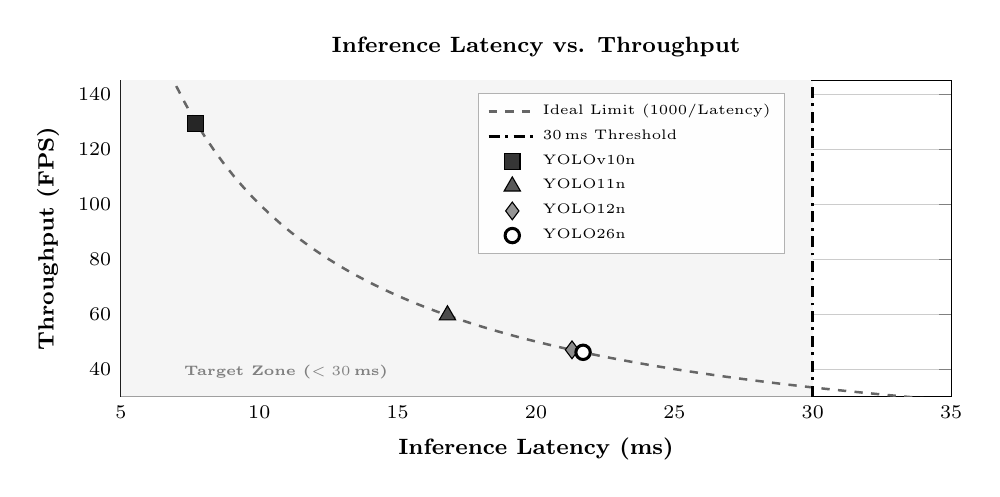
\begin{tikzpicture}
\begin{axis}[
  width=\columnwidth,
  height=5.6cm,
  title={Inference Latency vs. Throughput},
  title style={font=\footnotesize\bfseries, yshift=-1pt},
  xlabel={Inference Latency (ms)},
  ylabel={Throughput (FPS)},
  xmin=5, xmax=35,
  ymin=30, ymax=145,
  xtick={5, 10, 15, 20, 25, 30, 35},
  ytick={40, 60, 80, 100, 120, 140},
  grid=both,
  grid style={line width=0.1pt, draw=gray!25},
  major grid style={line width=0.25pt, draw=gray!40},
  tick label style={font=\scriptsize},
  label style={font=\footnotesize\bfseries},
  legend style={
    font=\tiny,
    at={(0.80, 0.96)},
    anchor=north east,
    draw=gray!60,
    fill=white,
    fill opacity=0.92,
    text opacity=1,
    cells={anchor=west}
  }
]
\addplot[fill=black!4, draw=none, forget plot] coordinates {(5,30) (30,30) (30,145) (5,145)} \closedcycle;
\node[font=\tiny\bfseries, text=black!50, anchor=south east] at (axis cs:15, 33) {Target Zone ($<30$\,ms)};
\addplot[
  domain=7.0:34,
  samples=80,
  dashed,
  color=black!60,
  line width=0.9pt
] {1000 / x};
\addlegendentry{Ideal Limit ($1000/\mathrm{Latency}$)}
\addplot[
  color=black,
  dash pattern=on 4pt off 2pt on 1pt off 2pt,
  line width=1.1pt
] coordinates {(30, 30) (30, 145)};
\addlegendentry{30\,ms Threshold}
\addplot[
  only marks,
  mark=square*,
  mark size=2.8pt,
  draw=black,
  fill=black!85
] coordinates {(7.7, 129.2)};
\addlegendentry{YOLOv10n}
\addplot[
  only marks,
  mark=triangle*,
  mark size=3.4pt,
  draw=black,
  fill=black!70
] coordinates {(16.8, 59.6)};
\addlegendentry{YOLO11n}
\addplot[
  only marks,
  mark=diamond*,
  mark size=3.2pt,
  draw=black,
  fill=black!45
] coordinates {(21.3, 47.0)};
\addlegendentry{YOLO12n}
\addplot[
  only marks,
  mark=*,
  mark size=2.6pt,
  draw=black,
  fill=white,
  line width=1.1pt
] coordinates {(21.7, 46.1)};
\addlegendentry{YOLO26n}
\end{axis}
\end{tikzpicture}
\caption{Inference latency versus throughput across evaluated YOLO models. Each model uses a distinct marker shape for clarity in greyscale printouts. All models achieve inference speeds within the 30\,ms edge requirement.}
\label{fig:latency_throughput}
\end{figure}

Fig.~\ref{fig:latency_throughput} shows measured latency and throughput alongside the theoretical limit ($\text{FPS} = 1000 / \text{latency}$) and the 30\,ms real-time ceiling. Peak GPU memory usage remained stable at approximately 1.5\,GB of VRAM across all four architectures.

\begin{figure*}[t]
\centering
\begin{tikzpicture}[
  scale=0.95,
  every node/.style={transform shape},
  font=\sffamily\footnotesize,
  box/.style={rectangle, draw=blue!70!black, fill=blue!5, thick, rounded corners=3pt, minimum height=0.9cm, align=center, inner sep=5pt},
  data/.style={rectangle, draw=gray!70, fill=gray!10, rounded corners=3pt, minimum height=0.9cm, align=center, inner sep=5pt},
  yolo/.style={rectangle, draw=orange!85!black, fill=orange!12, thick, rounded corners=3pt, minimum height=0.9cm, align=center, inner sep=5pt},
  arrow/.style={-{Stealth[scale=1.0]}, thick, color=gray!80!black},
  miningbox/.style={rectangle, draw=violet!80!black, fill=violet!8, thick, dashed, rounded corners=3pt, minimum height=0.9cm, align=center, inner sep=5pt},
  deploybox/.style={rectangle, draw=teal!80!black, fill=teal!10, line width=1.1pt, rounded corners=3pt, minimum height=0.9cm, align=center, inner sep=5pt},
  looparrow/.style={-{Stealth[scale=1.0]}, thick, color=violet!80!black, dashed}
]
\node[anchor=west, font=\bfseries\normalsize] at (0, 3.65) {(a) Localized Behavioral Cue Annotations vs. Baseline Negative};
\node[inner sep=0pt, outer sep=0pt] (img1) at (1.6, 1.65) {
  
\includegraphics[width=3.0cm, height=3.0cm]{figures/cue_yawn.jpg}
};
\draw[red!75!black, line width=1.4pt, solid] ($(img1.south west)!0.32!(img1.north west) + (img1.south west)!0.46!(img1.south east) - (img1.south west)$) rectangle ($(img1.south west)!0.46!(img1.north west) + (img1.south west)!0.67!(img1.south east) - (img1.south west)$) node[above right, fill=red!75!black, text=white, inner sep=1.5pt, font=\sffamily\tiny\bfseries] at ($(img1.south west)!0.46!(img1.north west) + (img1.south west)!0.46!(img1.south east) - (img1.south west)$) {yawn};
\node[below=3pt of img1, font=\sffamily\scriptsize\bfseries] {Yawning};

\node[inner sep=0pt, outer sep=0pt, right=0.45cm of img1] (img2) {
  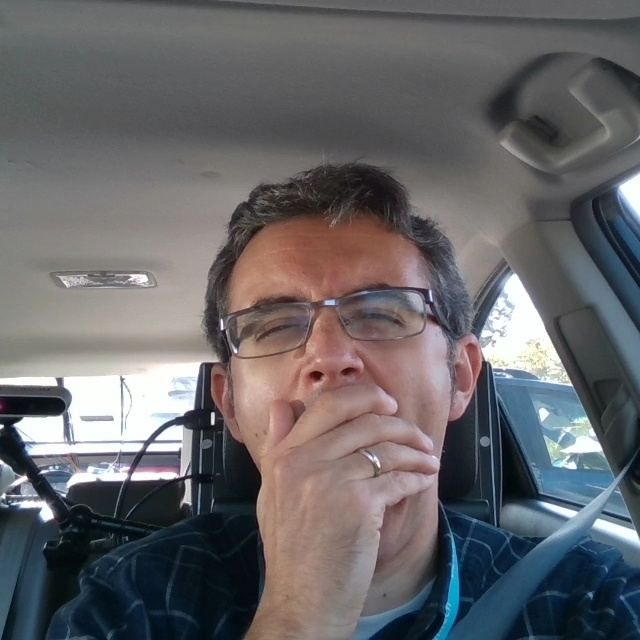
\includegraphics[width=3.0cm, height=3.0cm]{figures/cue_hand_mouth.jpg}
};
\draw[cyan!80!black, line width=1.4pt, densely dashed] ($(img2.south west)!0.05!(img2.north west) + (img2.south west)!0.38!(img2.south east) - (img2.south west)$) rectangle ($(img2.south west)!0.58!(img2.north west) + (img2.south west)!0.70!(img2.south east) - (img2.south west)$) node[above right, fill=cyan!80!black, text=white, inner sep=1.5pt, font=\sffamily\tiny\bfseries] at ($(img2.south west)!0.58!(img2.north west) + (img2.south west)!0.38!(img2.south east) - (img2.south west)$) {hand-mouth};
\node[below=3pt of img2, font=\sffamily\scriptsize\bfseries] {Hand-over-Mouth $^{\dagger}$};

\node[inner sep=0pt, outer sep=0pt, right=0.45cm of img2] (img3) {
  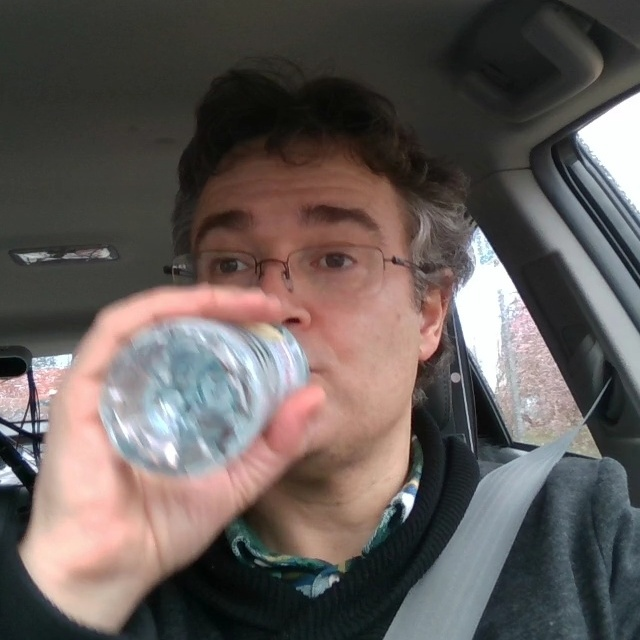
\includegraphics[width=3.0cm, height=3.0cm]{figures/cue_drink.jpg}
};
\draw[teal!80!black, line width=1.5pt, densely dotted] ($(img3.south west)!0.22!(img3.north west) + (img3.south west)!0.14!(img3.south east) - (img3.south west)$) rectangle ($(img3.south west)!0.56!(img3.north west) + (img3.south west)!0.49!(img3.south east) - (img3.south west)$) node[above right, fill=teal!80!black, text=white, inner sep=1.5pt, font=\sffamily\tiny\bfseries] at ($(img3.south west)!0.56!(img3.north west) + (img3.south west)!0.14!(img3.south east) - (img3.south west)$) {drink};
\node[below=3pt of img3, font=\sffamily\scriptsize\bfseries] {Drinking};

\node[inner sep=0pt, outer sep=0pt, right=0.45cm of img3] (img4) {
  
\includegraphics[width=3.0cm, height=3.0cm]{figures/cue_phone.jpg}
};
\draw[violet!85!black, line width=1.4pt, dashdotted] ($(img4.south west)!0.22!(img4.north west) + (img4.south west)!0.03!(img4.south east) - (img4.south west)$) rectangle ($(img4.south west)!0.63!(img4.north west) + (img4.south west)!0.28!(img4.south east) - (img4.south west)$) node[above right, fill=violet!85!black, text=white, inner sep=1.5pt, font=\sffamily\tiny\bfseries] at ($(img4.south west)!0.63!(img4.north west) + (img4.south west)!0.03!(img4.south east) - (img4.south west)$) {phone};
\node[below=3pt of img4, font=\sffamily\scriptsize\bfseries] {Phone Use};

\node[inner sep=0pt, outer sep=0pt, right=0.45cm of img4] (img5) {
  
\includegraphics[width=3.0cm, height=3.0cm]{figures/cue_negative.jpg}
};
\node[above left, fill=gray!80!black, text=white, inner sep=2pt, font=\sffamily\tiny\bfseries, rounded corners=1pt] at ($(img5.north east) + (-0.08, -0.28)$) {No Cue};
\node[below=3pt of img5, font=\sffamily\scriptsize\bfseries] {Negative (Baseline)};

\draw[gray!35, line width=0.8pt] (0, -0.35) -- (17.5, -0.35);

\node[anchor=west, font=\bfseries\normalsize] at (0, -0.75) {(b) Training Pipeline and Closed-Loop Hard-Negative Mining};
\node[data, text width=2.3cm] (raw) at (1.3, -1.9) {\textbf{DMD Stream}\\15,723 Frames\\(1 FPS Extraction)};
\node[data, text width=2.6cm, right=0.6cm of raw] (split) {\textbf{Core Partition}\\Positives: 2,401\\Neg. Pool: 10,178};
\node[box, text width=2.4cm, right=0.6cm of split] (ratios) {\textbf{RQ1: Sweep Ratios}\\0\%, 20\%, 40\%,\\60\%, 80\%};
\node[yolo, text width=2.5cm, right=0.6cm of ratios] (yolo) {\textbf{Train Detectors}\\Lightweight YOLO\\(Edge-Ready)};
\node[data, text width=2.6cm, right=0.6cm of yolo] (eval) {\textbf{Held-Out Eval}\\Val \& Test Streams\\(80.9\% Negative)};

\node[miningbox, text width=3.4cm] (mining) at ($(split.south)!0.5!(ratios.south) + (0, -1.65)$) {\textbf{RQ2: Hard Mining}\\Harvest FPs from\\Train Negative Pool};
\node[deploybox, text width=2.8cm, below=1.2cm of eval] (deploy) {\textbf{In-Cabin Deploy}\\Sub-30\,ms Latency\\Low Alert Rate ($\mathcal{A}_h$)};

\draw[arrow] (raw) -- (split);
\draw[arrow] (split) -- (ratios);
\draw[arrow] (ratios) -- (yolo);
\draw[arrow] (yolo) -- (eval);
\draw[-{Stealth[scale=1.0]}, very thick, color=teal!75!black] (eval.south) -- node[right, font=\tiny\bfseries, text=teal!75!black] {Verified} (deploy.north);
\draw[-{Stealth[scale=1.0]}, thick, color=violet!80!black, dashdotdotted] (yolo.south) |- (mining.east) node[pos=0.35, right, font=\tiny\bfseries, text=violet!80!black, xshift=2pt] {Mine Neg. Pool};
\draw[looparrow] (mining.north) -- (split.south) node[midway, left, font=\tiny\bfseries, text=violet!80!black, xshift=-4pt] {Inject Hard Negs};
\end{tikzpicture}
\caption{Overview of the training and deployment pipeline: (a) Target behavioral cues ($640 \times 640$ pixels) with an unannotated negative frame (baseline driving). When a driver covers a yawn, the action is labeled as hand-over-mouth ($^{\dagger}$). Line styles and colors provide dual encoding for greyscale clarity. (b) The training pipeline evaluates negative frame ratios and harvests FPs to retrain the model, reducing nuisance alert rates ($\mathcal{A}_h$) for in-cabin driver monitoring systems (DMS).}
\label{fig:combined_framework}
\end{figure*}

\begin{table}[htbp]
\caption{Dataset Splits and Frame Distributions}
\begin{center}
\begin{tabular}{|c|c|c|c|}
\hline
\textbf{Split} & \multicolumn{3}{|c|}{\textbf{Frame Counts}} \\
\cline{2-4}
& \textbf{\textit{Positive}} & \textbf{\textit{Negative}} & \textbf{\textit{Total}} \\
\hline
0\%                 & 2,401 & 0     & 2,401  \\
20\%                & 2,401 & 600   & 3,001  \\
40\%                & 2,401 & 1,600 & 4,001  \\
60\%                & 2,401 & 3,602 & 6,003  \\
80\%                & 2,401 & 9,604 & 12,005 \\
\hline
Val $^{\dagger}$      & 300   & 1,272 & 1,572  \\
Test $^{\dagger}$     & 300   & 1,272 & 1,572  \\
\hline
\multicolumn{4}{l}{$^{\dagger}$ Evaluation sets feature an 80.9\% negative ratio.}
\end{tabular}
\label{tab:splits}
\end{center}
\end{table} % DONE 
\section{Experimental Results}

\subsection{Negative-to-Positive Ratio Sweep}
\label{subsec:results_ratio}
To address RQ1, we evaluate how the proportion of negative training frames affects cue detection accuracy and false-alarm suppression. We train each detector across the five negative-frame ratios in Table~\ref{tab:splits}: 0\%, 20\%, 40\%, 60\%, and 80\%, corresponding to negative-to-positive frame ratios of $0:1$, $0.25:1$, $0.67:1$, $1.50:1$, and $4.00:1$. Fig.~\ref{fig:ratio_sweep} reports detection metrics and false-positive rates on the held-out test set (1,272 negative frames).

\begin{figure}[htbp]
\centering
\pgfplotslegendfromname{leg_ratio_sweep}\\[2pt]
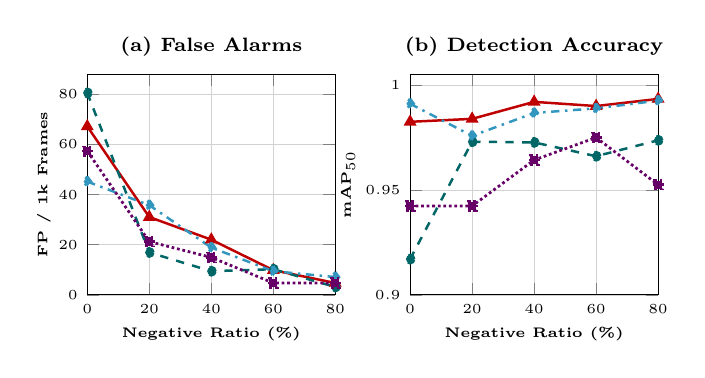
\begin{tikzpicture}
\begin{axis}[
  name=p1,
  scale only axis,
  width=3.15cm, height=2.8cm,
  title={(a) False Alarms},
  title style={font=\scriptsize\bfseries, yshift=-3pt},
  xlabel={Negative Ratio (\%)},
  ylabel={FP / 1k Frames},
  xlabel style={font=\tiny\bfseries, yshift=2pt},
  ylabel style={font=\tiny\bfseries, yshift=-4pt},
  tick label style={font=\tiny},
  xmin=0, xmax=80,
  ymin=0, ymax=88,
  xtick={0, 20, 40, 60, 80},
  ytick={0, 20, 40, 60, 80},
  grid=both,
  grid style={line width=0.1pt, draw=gray!20},
  major grid style={line width=0.2pt, draw=gray!35},
  legend to name=leg_ratio_sweep,
  legend style={
    font=\tiny,
    draw=gray!50,
    fill=white,
    cells={anchor=west},
    legend columns=4,
    column sep=4pt,
    inner sep=2pt
  }
]
\addplot[
  color=red!75!black,
  line width=0.9pt,
  solid,
  mark=triangle*,
  mark size=1.8pt
] coordinates { (0, 67.22) (20, 31.05) (40, 22.01) (60, 9.83) (80, 4.72) };
\addlegendentry{YOLO11n}

\addplot[
  color=teal!80!black,
  line width=0.9pt,
  dashed,
  mark=*,
  mark size=1.5pt
] coordinates { (0, 80.59) (20, 16.90) (40, 9.43) (60, 10.22) (80, 3.14) };
\addlegendentry{YOLO26n}

\addplot[
  color=cyan!75!black,
  line width=0.9pt,
  dashdotted,
  mark=diamond*,
  mark size=1.8pt
] coordinates { (0, 45.20) (20, 35.77) (40, 18.86) (60, 9.43) (80, 7.08) };
\addlegendentry{YOLO12n}

\addplot[
  color=violet!80!black,
  line width=1.0pt,
  densely dotted,
  mark=square*,
  mark size=1.5pt
] coordinates { (0, 57.39) (20, 21.23) (40, 14.94) (60, 4.72) (80, 4.72) };
\addlegendentry{YOLOv10n}
\end{axis}

\begin{axis}[
  name=p2,
  at={($(p1.east) + (0.95cm, 0)$)},
  anchor=west,
  scale only axis,
  width=3.15cm, height=2.8cm,
  title={(b) Detection Accuracy},
  title style={font=\scriptsize\bfseries, yshift=-3pt},
  xlabel={Negative Ratio (\%)},
  ylabel={$\text{mAP}_{50}$},
  xlabel style={font=\tiny\bfseries, yshift=2pt},
  ylabel style={font=\tiny\bfseries, yshift=-3pt},
  tick label style={font=\tiny},
  xmin=0, xmax=80,
  ymin=0.90, ymax=1.005,
  xtick={0, 20, 40, 60, 80},
  ytick={0.90, 0.95, 1.00},
  yticklabel style={/pgf/number format/fixed, /pgf/number format/precision=2},
  grid=both,
  grid style={line width=0.1pt, draw=gray!20},
  major grid style={line width=0.2pt, draw=gray!35}
]
\addplot[
  color=red!75!black,
  line width=0.9pt,
  solid,
  mark=triangle*,
  mark size=1.8pt
] coordinates { (0, 0.9824) (20, 0.9838) (40, 0.9919) (60, 0.9899) (80, 0.9933) };
\addplot[
  color=teal!80!black,
  line width=0.9pt,
  dashed,
  mark=*,
  mark size=1.5pt
] coordinates { (0, 0.9170) (20, 0.9729) (40, 0.9726) (60, 0.9660) (80, 0.9736) };
\addplot[
  color=cyan!75!black,
  line width=0.9pt,
  dashdotted,
  mark=diamond*,
  mark size=1.8pt
] coordinates { (0, 0.9910) (20, 0.9757) (40, 0.9866) (60, 0.9888) (80, 0.9925) };
\addplot[
  color=violet!80!black,
  line width=1.0pt,
  densely dotted,
  mark=square*,
  mark size=1.5pt
] coordinates { (0, 0.9423) (20, 0.9423) (40, 0.9642) (60, 0.9749) (80, 0.9524) };
\end{axis}
\end{tikzpicture}
\caption{Impact of negative-to-positive curation ratios (RQ1): (a) false alarms per 1{,}000 frames (FP/1k) exhibit an overall downward trajectory across all models as negative ratios increase (converging at 80\% despite a transient rise for YOLO26n between 40\% and 60\%); (b) core detection accuracy ($\text{mAP}_{50}$) remains stable. Distinct marker shapes and line styles ensure readability in greyscale.}
\label{fig:ratio_sweep}
\end{figure}

\textbf{High-Ratio Convergence:} As shown in Fig.~\ref{fig:ratio_sweep}, models trained without negative frames (0\%) generate high false-alarm rates, ranging from 45.20 to 80.59\,FP/1k. Increasing the negative ratio to 80\% reduces false alarms across all four architectures, converging to between 3.14 and 7.08\,FP/1k. This represents a $6.4\times$ to $25.7\times$ reduction in false alarms relative to the 0\% baseline. Across all 20 evaluated configurations, negative ratio shows a strong inverse correlation with FP/1k (Spearman $\rho = -0.937, p < 10^{-4}$).

\textbf{Cue Sensitivity and Localization Stability:} Precision improves with negative ratio (Spearman $\rho = +0.546, p < 0.05$), driven directly by the reduction in false alarms. Recall remains uncorrelated with negative ratio (Spearman $\rho = +0.012, p > 0.50$), showing that background negative frames do not cause under-detection. Localization accuracy ($\text{mAP}_{50:95}$) remains stable across all splits, ranging between 0.7086 and 0.7766.

\textbf{Trajectory Divergence at Intermediate Ratios:} While all models converge at 80\% negatives, their trajectories differ between 20\% and 60\%. YOLO26n drops from 80.59 to 16.90\,FP/1k at 20\% negatives, achieving early suppression. In contrast, YOLO11n, YOLO12n, and YOLOv10n show a more gradual decline, requiring ratios between 60\% and 80\% to reach comparable false-alarm rates.

\begin{figure*}[t]
\centering
\definecolor{c11n}{RGB}{31,119,180}
\definecolor{c26n}{RGB}{214,39,40}
\definecolor{c12n}{RGB}{44,160,44}
\definecolor{c10n}{RGB}{255,127,14}
\begin{tikzpicture}
\begin{axis}[
  scale only axis,
  width=0.85\textwidth,
  height=6.2cm,
  xlabel={Negative Ratio (\%)},
  ylabel={FP/1k (measured, log scale)},
  xtick={0,20,40,60,80},
  xmin=0, xmax=95,
  ymode=log,
  ymin=2, ymax=100,
  axis y line*=left,
  legend style={
    font=\scriptsize,
    at={(0.98,0.98)},
    anchor=north east,
    draw=gray!60,
    fill=white,
    fill opacity=0.92,
    text opacity=1,
    inner sep=3pt,
    row sep=1.5pt
  },
  legend cell align={left},
  title={False-Alarm Rate and Projected Nuisance Alerts vs. Negative Ratio},
  title style={font=\footnotesize\bfseries}
]
% --- Swept Curves: Randomly Sampled Negatives ---
\addplot[color=c11n, mark=square*, mark size=2.2pt, thick] coordinates {(0,67.22)(20,31.05)(40,22.01)(60,9.83)(80,4.72)};
\addlegendentry{YOLO11n (Randomly Sampled)}

\addplot[color=c26n, mark=triangle*, mark size=2.6pt, thick] coordinates {(0,80.59)(20,16.90)(40,9.43)(60,10.22)(80,3.14)};
\addlegendentry{YOLO26n (Randomly Sampled)}

\addplot[color=c12n, mark=diamond*, mark size=2.4pt, thick] coordinates {(0,45.20)(20,35.77)(40,18.86)(60,9.43)(80,7.08)};
\addlegendentry{YOLO12n (Randomly Sampled)}

\addplot[color=c10n, mark=*, mark size=2.0pt, thick] coordinates {(0,57.39)(20,21.23)(40,14.94)(60,4.72)(80,4.72)};
\addlegendentry{YOLOv10n (Randomly Sampled)}

% --- 40% Hard-Mined Stars ---
\addplot[only marks, mark=star, mark size=5.2pt, line width=1.2pt, color=c11n] coordinates {(37.0,7.08)};
\addplot[only marks, mark=star, mark size=5.2pt, line width=1.2pt, color=c26n] coordinates {(39.0,6.29)};
\addplot[only marks, mark=star, mark size=5.2pt, line width=1.2pt, color=c12n] coordinates {(41.0,6.29)};
\addplot[only marks, mark=star, mark size=5.2pt, line width=1.2pt, color=c10n] coordinates {(43.0,7.08)};

\addlegendimage{only marks, mark=star, mark size=5.2pt, line width=1.2pt, color=black}
\addlegendentry{40\% Hard-Mined}

% --- Leader Lines to Callout Badges ---
\draw[color=c11n, line width=0.6pt, -{Stealth[scale=0.6]}] (axis cs:32.8, 4.3) -- (axis cs:36.4, 6.6);
\draw[color=c26n, line width=0.6pt, -{Stealth[scale=0.6]}] (axis cs:37.5, 3.2) -- (axis cs:38.7, 5.6);
\draw[color=c12n, line width=0.6pt, -{Stealth[scale=0.6]}] (axis cs:42.5, 3.2) -- (axis cs:41.3, 5.6);
\draw[color=c10n, line width=0.6pt, -{Stealth[scale=0.6]}] (axis cs:47.2, 4.3) -- (axis cs:43.6, 6.6);

% --- Model Callout Badges ---
\node[font=\tiny\bfseries, text=c11n, fill=white, draw=c11n!70, rounded corners=1.5pt, inner sep=1.2pt] at (axis cs:32.0, 3.7) {11n};
\node[font=\tiny\bfseries, text=c26n, fill=white, draw=c26n!70, rounded corners=1.5pt, inner sep=1.2pt] at (axis cs:37.0, 2.7) {26n};
\node[font=\tiny\bfseries, text=c12n, fill=white, draw=c12n!70, rounded corners=1.5pt, inner sep=1.2pt] at (axis cs:43.0, 2.7) {12n};
\node[font=\tiny\bfseries, text=c10n, fill=white, draw=c10n!70, rounded corners=1.5pt, inner sep=1.2pt] at (axis cs:48.0, 3.7) {v10n};
\end{axis}

\begin{axis}[
  scale only axis,
  width=0.85\textwidth,
  height=6.2cm,
  hide x axis,
  ymode=log,
  ymin=174.7, ymax=8737,
  ytick={200,500,1000,2000,5000},
  minor tick num=0,
  axis y line*=right,
  ylabel={Alerts/hr (30\,FPS, derived)},
]
\end{axis}
\end{tikzpicture}
\caption{False-positive rate (left axis, measured) and projected hourly nuisance alerts at 30\,FPS (right axis, derived via~\eqref{eq:ah}) as a function of negative-frame ratio. Solid curves track uniform random negative curation, while individual stars denote each model's 40\% hard-negative-mined configuration.}
\label{fig:results_combined}
\end{figure*}
\subsection{Hard-Negative Mining vs. Random Negatives}
\label{subsec:results_curation}
To address RQ2, we evaluate whether replacing randomly sampled negatives with hard negatives improves false-alarm suppression at matched dataset size. Following Section~\ref{subsec:mining}, we extract false positives produced by the 0\% baseline detector at $\tau = 0.25$, backfilling with random negatives to reach $N_{\mathrm{target}} = 1{,}600$ negative frames (4,001 total frames, matching the 40\% reference ratio). Fig.~\ref{fig:hard_mining_bars} compares two-seed sample means ($\text{seed} \in \{42, 43\}$) for random negative sampling versus hard-negative mining.

\begin{figure}[htbp]
\centering
\pgfplotslegendfromname{leg_mining}\\[2pt]
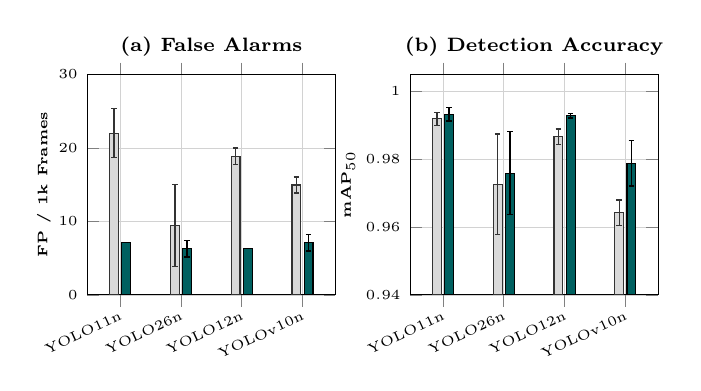
\begin{tikzpicture}
\begin{axis}[
  name=p1,
  ybar=1.2pt,
  bar width=3.2pt,
  scale only axis,
  width=3.15cm, height=2.8cm,
  title={(a) False Alarms},
  title style={font=\scriptsize\bfseries, yshift=-3pt},
  ylabel={FP / 1k Frames},
  xlabel style={font=\tiny\bfseries, yshift=2pt},
  ylabel style={font=\tiny\bfseries, yshift=-4pt},
  tick label style={font=\tiny},
  symbolic x coords={YOLO11n, YOLO26n, YOLO12n, YOLOv10n},
  xtick=data,
  xticklabel style={font=\tiny, rotate=25, anchor=north east, inner sep=1pt},
  enlarge x limits=0.18,
  ymin=0, ymax=30,
  ytick={0, 10, 20, 30},
  grid=both,
  grid style={line width=0.1pt, draw=gray!20},
  major grid style={line width=0.2pt, draw=gray!35},
  legend to name=leg_mining,
  legend style={
    font=\tiny,
    draw=gray!50,
    fill=white,
    cells={anchor=west},
    legend columns=2,
    column sep=6pt,
    inner sep=2pt
  }
]
\addplot[
  fill=gray!30,
  draw=black!80,
  error bars/.cd,
  y dir=both,
  y explicit,
  error bar style={line width=0.5pt, color=black!80},
  error mark options={rotate=90, mark size=1pt, line width=0.5pt}
] coordinates {
  (YOLO11n, 22.01)  +- (0, 3.34)
  (YOLO26n, 9.43)   +- (0, 5.56)
  (YOLO12n, 18.86)  +- (0, 1.11)
  (YOLOv10n, 14.94) +- (0, 1.11)
};
\addlegendentry{Random Negatives (40\%)}

\addplot[
  fill=teal!75!black,
  draw=black,
  error bars/.cd,
  y dir=both,
  y explicit,
  error bar style={line width=0.5pt, color=black},
  error mark options={rotate=90, mark size=1pt, line width=0.5pt}
] coordinates {
  (YOLO11n, 7.08)  +- (0, 0.00)
  (YOLO26n, 6.29)  +- (0, 1.12)
  (YOLO12n, 6.29)  +- (0, 0.00)
  (YOLOv10n, 7.08) +- (0, 1.11)
};
\addlegendentry{Hard-Negative Mining (40\%)}
\end{axis}

\begin{axis}[
  name=p2,
  at={($(p1.east) + (0.95cm, 0)$)},
  anchor=west,
  ybar=1.2pt,
  bar width=3.2pt,
  scale only axis,
  width=3.15cm, height=2.8cm,
  title={(b) Detection Accuracy},
  title style={font=\scriptsize\bfseries, yshift=-3pt},
  ylabel={$\text{mAP}_{50}$},
  xlabel style={font=\tiny\bfseries, yshift=2pt},
  ylabel style={font=\tiny\bfseries, yshift=-3pt},
  tick label style={font=\tiny},
  symbolic x coords={YOLO11n, YOLO26n, YOLO12n, YOLOv10n},
  xtick=data,
  xticklabel style={font=\tiny, rotate=25, anchor=north east, inner sep=1pt},
  enlarge x limits=0.18,
  ymin=0.94, ymax=1.005,
  ytick={0.94, 0.96, 0.98, 1.00},
  yticklabel style={/pgf/number format/fixed, /pgf/number format/precision=2},
  grid=both,
  grid style={line width=0.1pt, draw=gray!20},
  major grid style={line width=0.2pt, draw=gray!35}
]
\addplot[
  fill=gray!30,
  draw=black!80,
  error bars/.cd,
  y dir=both,
  y explicit,
  error bar style={line width=0.5pt, color=black!80},
  error mark options={rotate=90, mark size=1pt, line width=0.5pt}
] coordinates {
  (YOLO11n, 0.9919)  +- (0, 0.0019)
  (YOLO26n, 0.9726)  +- (0, 0.0148)
  (YOLO12n, 0.9866)  +- (0, 0.0023)
  (YOLOv10n, 0.9642) +- (0, 0.0037)
};
\addplot[
  fill=teal!75!black,
  draw=black,
  error bars/.cd,
  y dir=both,
  y explicit,
  error bar style={line width=0.5pt, color=black},
  error mark options={rotate=90, mark size=1pt, line width=0.5pt}
] coordinates {
  (YOLO11n, 0.9932)  +- (0, 0.0020)
  (YOLO26n, 0.9759)  +- (0, 0.0122)
  (YOLO12n, 0.9928)  +- (0, 0.0007)
  (YOLOv10n, 0.9788) +- (0, 0.0067)
};
\end{axis}
\end{tikzpicture}
\caption{Hard-negative mining versus random negative sampling ($r_{\mathrm{ref}} = 40\%$, RQ2): (a) false alarms per 1{,}000 frames (FP/1k) decrease under hard mining across all architectures; (b) core detection accuracy ($\text{mAP}_{50}$) remains stable. Bars reflect two-seed means with error bars indicating $\pm 1$ standard deviation.}
\label{fig:hard_mining_bars}
\end{figure}

\textbf{Architectural Variations in Suppression:} As shown in Fig.~\ref{fig:hard_mining_bars}, hard-negative mining lowers FP/1k across all four models, with distinct responses across architectures:
\begin{itemize}
    \item \textit{Attention and Dual-Assignment Models:} YOLO11n, YOLO12n, and YOLOv10n show substantial false-alarm reductions: $-67.8\%$ for YOLO11n ($22.01 \to 7.08$\,FP/1k), $-66.7\%$ for YOLO12n ($18.86 \to 6.29$\,FP/1k), and $-52.6\%$ for YOLOv10n ($14.94 \to 7.08$\,FP/1k). Localization quality also improves, with $\text{mAP}_{50:95}$ increasing by up to $+0.018$ in YOLO12n.
    \item \textit{Convolutional Models:} In comparison, YOLO26n shows a smaller reduction of $-33.3\%$ ($9.43 \to 6.29$\,FP/1k), indicating diminishing returns from hard mining relative to random background frames.
\end{itemize}

\subsection{Nuisance Alert Projection}
\label{subsec:results_nuisance}
To evaluate operational reliability, we project measured false-alarm rates into expected hourly nuisance alerts ($\mathcal{A}_h$) using~\eqref{eq:ah}. In natural driving, target distraction events are infrequent, with baseline driving accounting for $p_{\mathrm{neg}} \approx 0.809$ (80.9\%) of operational frames. Table~\ref{tab:nuisance_alerts} reports projected alert rates across three streaming rates: 5\,FPS (low-power sampling), 15\,FPS (standard embedded vision), and 30\,FPS (full real-time streaming).

\begin{table}[t]
\caption{Projected Nuisance Alerts per Hour ($\mathcal{A}_h$) Across Negative Ratios and Frame Rates}
\label{tab:nuisance_alerts}
\begin{center}
\setlength{\tabcolsep}{4.0pt}
\begin{tabular}{|l|l|c|c|c|}
\hline
\textbf{Model} & \textbf{Training Configuration} & \textbf{5\,FPS} & \textbf{15\,FPS} & \textbf{30\,FPS} \\
\hline
\multirow{4}{*}{YOLO11n}
& 0\% Baseline        & 979     & 2{,}937 & 5{,}873 \\
& 40\% Random         & 321     & 962     & 1{,}923 \\
& 40\% Hard-Mined     & 103     & 309     & 619     \\
& 80\% Ratio          & \textbf{69} & \textbf{206} & \textbf{412} \\
\hline
\multirow{4}{*}{YOLO26n}
& 0\% Baseline        & 1{,}174 & 3{,}521 & 7{,}041 \\
& 40\% Random         & 137     & 412     & 824     \\
& 40\% Hard-Mined     & 92      & 275     & 550     \\
& 80\% Ratio          & \textbf{46} & \textbf{137} & \textbf{274} \\
\hline
\multirow{4}{*}{YOLO12n}
& 0\% Baseline        & 658     & 1{,}975 & 3{,}949 \\
& 40\% Random         & 275     & 824     & 1{,}648 \\
& 40\% Hard-Mined     & \textbf{92} & \textbf{275} & \textbf{550} \\
& 80\% Ratio          & 103     & 309     & 619     \\
\hline
\multirow{4}{*}{YOLOv10n}
& 0\% Baseline        & 836     & 2{,}507 & 5{,}014 \\
& 40\% Random         & 218     & 653     & 1{,}305 \\
& 40\% Hard-Mined     & 103     & 309     & 619     \\
& 80\% Ratio          & \textbf{69} & \textbf{206} & \textbf{412} \\
\hline
\end{tabular}
\end{center}
\vspace{-1pt}
{\footnotesize Projected via~\eqref{eq:ah} using $\mathcal{A}_h = 3.6 \times r \times p_{\mathrm{neg}} \times \text{FP/1k}$ with natural negative prevalence $p_{\mathrm{neg}} = 0.809$. Inputs correspond to Fig.~\ref{fig:ratio_sweep} and Fig.~\ref{fig:hard_mining_bars}. Bold indicates the lowest alert rate per architecture.}
\end{table}

\textbf{Alert Frequency and Automation Disuse:} As detailed in Table~\ref{tab:nuisance_alerts}, models trained without negative frames (0\%) produce impractically high false-alarm rates. At 30\,FPS, unregularized models trigger between 3{,}949 and 7{,}041 nuisance alerts per hour, averaging 1 to 2 false detections per second. At 5\,FPS, baseline models trigger 658 to 1{,}174 false alerts per hour. Frequent false alarms lead directly to alert fatigue and automation disuse \cite{lambert2026chinese, parasuraman1997humans}.

\textbf{Secondary Compute and Thermal Load:} Frequent false alarms trigger downstream tracking routines continuously, creating processing spikes that risk thermal throttling on embedded chips \cite{florez2024real, benoitcattin2020thermal}.

\textbf{Mitigation via Negative Curation:} Scaling negative training frames reduces projected alert rates by up to 96.1\%. At 80\% negative prevalence, alert rates decline to 274--619\,alerts/hr at 30\,FPS and 46--103\,alerts/hr at 5\,FPS. Table~\ref{tab:nuisance_alerts} also indicates that targeted hard-negative mining achieves comparable suppression at half the negative volume: at a 40\% ratio, hard-mined models produce 550--619\,alerts/hr at 30\,FPS, reducing baseline alerts by over 84\%.

These projections highlight an engineering distinction: \textit{inference latency depends on architecture, whereas operational reliability depends on curation}. While all four models achieve real-time execution speeds (7.7--21.7\,ms, Fig.~\ref{fig:latency_throughput}), data curation determines whether a lightweight detector can operate without triggering alert fatigue or thermal throttling.
% DONE
\section{Discussion}

\subsection{Architectural Mechanisms and Practical Curation Guidelines}
\label{subsec:guidelines}
Our empirical findings reveal that a detector's internal feature-aggregation mechanism influences its response to negative-frame curation:

\textbf{Mechanistic Comparison:} Random negative sampling predominantly selects low-entropy background patches that produce small loss gradients. For convolutional architectures like YOLO26n, localized $3 \times 3$ re-parameterized convolution (RepConv) kernels suppress repetitive cabin textures using uniform background frames. Consequently, YOLO26n reaches an early suppression plateau at 20\% negatives and derives modest benefit from hard mining ($-33.3\%$).

In contrast, architectures using self-attention (YOLO11n), area attention (YOLO12n), or dual-label assignment (YOLOv10n) model wider spatial dependencies. Without background exposure, attention layers can correlate ambient artifacts, such as lighting glare or cabin contours, with target cues. Mined hard negatives provide high-entropy distractors that help attention projection heads separate cabin geometry from true driver cues. For YOLOv10n, mined negatives also penalize over-assignment in the auxiliary head, sharpening the decision boundary of the primary inference branch.

\textbf{Per-Seed Stability and Saturation:} Attention-equipped models (YOLO11n, YOLO12n) and dual-assignment architectures (YOLOv10n) demonstrate consistent metrics across random seeds. In contrast, YOLO26n exhibits seed-dependent sensitivity, with reductions ranging from 0.0\% under Seed~42 to 47.0\% under Seed~43.

\textbf{Practical Curation Guidelines:} These findings provide two engineering guidelines for edge DMS pipelines:
\begin{enumerate}
    \item \textit{Curate for Attention, Sample for Convolutions:} Systems deploying purely convolutional backbones achieve sufficient suppression through uniform random background sampling. Conversely, systems employing attention-centric or dual-assignment backbones should prioritize hard-negative mining, unlocking 52.6\% to 67.8\% additional false-alarm suppression at matched training compute.
    \item \textit{Prevalence Trade-offs (40\% vs. 80\%):} When training budgets permit larger datasets, an 80\% negative ratio ($4.00:1$ ratio) achieves the lowest false-alarm floor for most architectures (3.14--4.72\,FP/1k), though attention-based models such as YOLO12n achieve their lowest floor under 40\% hard mining (6.29\,FP/1k vs. 7.08\,FP/1k at 80\%). Where training compute or iteration time is constrained, a 40\% ratio curated with hard negatives delivers comparable suppression (6.29--7.08\,FP/1k) with one-third the total dataset volume (and one-sixth the negative frames).
\end{enumerate}
\subsection{Limitations}
\label{subsec:limitations}
This study has three primary limitations. First, a single annotator labeled the dataset without an independent second annotator to measure inter-annotator agreement. Although the protocol enforced strict mutual exclusion, ambiguous cases may reflect individual bias.

Second, the evaluation is limited to RGB video feeds. Commercial systems frequently use near-infrared (NIR) or depth cameras to maintain reliability under low-light conditions. Consequently, our benchmarks do not account for sensor-specific noise patterns or active infrared illumination.

Finally, we evaluate isolated per-frame inference without temporal smoothing, such as Kalman filtering or multi-frame consensus. Because production systems typically require detections to persist across consecutive frames before issuing a warning, our projected alert rates ($\mathcal{A}_h$) represent an unmitigated baseline rather than a complete multi-stage tracking pipeline.% DONE
\section{Conclusion} % DONE
This study evaluated negative-frame curation and hard-negative mining to suppress false alarms in lightweight, edge-deployed Driver Monitoring Systems (DMS). Across four You Only Look Once (YOLO) architectures with fewer than 3~million parameters, increasing the negative-to-positive training ratio from 0\% to 80\% reduced false positives per 1{,}000 frames (FP/1k) by $6.4\times$ to $25.7\times$. Core detection sensitivity ($\text{mAP}_{50:95}$), precision, and recall remained stable across all ratios. At a matched dataset volume, replacing random background frames with hard-mined false positives yielded an additional 33.3\% to 67.8\% false-alarm reduction. Attention-based models (YOLO11n, YOLO12n) and dual-assignment architectures (YOLOv10n) achieved the largest gains from hard mining, whereas the purely convolutional model (YOLO26n) reached early suppression using random negative frames alone. In operational driving projections, these curation strategies reduced projected nuisance alerts from thousands per hour to under 620\,alerts/hr at 30\,FPS, directly curbing driver alert fatigue and embedded computational load.

These findings show that negative-frame curation is as vital as model architecture for reliable edge deployment. Furthermore, curation strategies must match a detector's internal feature-aggregation mechanism: attention heads require high-entropy mined distractors to eliminate false correlations, whereas convolutional kernels regularize effectively on uniform background scenes. Despite these gains, this study has three shortcomings: the ground truth was produced by a single annotator, evaluations were conducted on isolated single-frame RGB feeds without temporal filtering, and hard-negative mining was restricted to a single closed-loop pass. Future work will extend these curation protocols to multi-modal near-infrared and depth feeds, integrate multi-frame temporal consensus into the alert projection, and evaluate iterative hard-negative mining across multiple training rounds.
\begin{thebibliography}{17}
\sloppy
\bibitem{ec2026safercars} European Commission, ``Type-approval requirements for general vehicle safety and the protection of vulnerable road users,'' \emph{Official Journal of the European Union}, Regulation (EU) 2019/2144, Commission Delegated Regulation (EU) 2021/1341, and Regulation (EU) 2023/2590, 2021--2023.
\bibitem{ortega2020dmd} J.~D. Ortega, N.~Kose, P.~Ca\~{n}as, M.-A. Chao, A.~Unnervik, M.~Nieto, O.~Otaegui, and L.~Salgado, ``DMD: A large-scale multi-modal driver monitoring dataset for attention and alertness analysis,'' in \emph{Proc. Eur. Conf. Comput. Vis. (ECCV) Workshops}, 2020, pp.~387--405.
\bibitem{florez2024real} R.~Florez, F.~Palomino-Quispe, A.~B. Alvarez, R.~J. Coaquira-Castillo, and J.~C. Herrera-Levano, ``A real-time embedded system for driver drowsiness detection based on visual analysis of the eyes and mouth using convolutional neural network and mouth aspect ratio,'' \emph{Sensors}, vol.~24, no.~19, Art. no.~6261, Sep. 2024, doi: 10.3390/s24196261.
\bibitem{liu2019edge} S.~Liu, L.~Liu, J.~Tang, B.~Yu, Y.~Wang, and W.~Shi, ``Edge computing for autonomous driving: Opportunities and challenges,'' \emph{Proc. IEEE}, vol.~107, no.~8, pp.~1697--1716, Aug. 2019, doi: 10.1109/JPROC.2019.2915983.
\bibitem{lambert2026chinese} F.~Lambert, ``Chinese drivers are using plastic heads to fool Tesla's Autopilot cabin camera,'' \emph{Electrek}, Jun.~15, 2026. [Online]. Available: \url{https://electrek.co/2026/06/15/chinese-drivers-plastic-heads-fool-tesla-autopilot-camera/}. [Accessed: Sep.~6, 2026].
\bibitem{benoitcattin2020thermal} T.~Benoit-Cattin, D.~Velasco-Montero, and J.~Fern\'{a}ndez-Berni, ``Impact of thermal throttling on long-term visual inference in a CPU-based edge device,'' \emph{Electronics}, vol.~9, no.~12, Art. no.~2106, 2020, doi: 10.3390/electronics9122106.
\bibitem{martin2019drive} M.~Martin, A.~Roitberg, M.~Haurilet, M.~Horne, S.~Rei{\ss}, M.~Peng, and R.~Stiefelhagen, ``Drive\&Act: A multi-modal dataset for fine-grained driver behavior recognition in autonomous vehicles,'' in \emph{Proc. IEEE/CVF Int. Conf. Comput. Vis. (ICCV)}, 2019, pp.~2801--2810.
\bibitem{canas2021detection} P.~Ca\~{n}as, J.~D. Ortega, M.~Nieto, and O.~Otaegui, ``Detection of distraction-related actions on DMD: An image and a video-based approach comparison,'' in \emph{Proc. Int. Conf. Comput. Vis. Theory Appl. (VISAPP)}, 2021, pp.~458--465.
\bibitem{yolodrive2025} H.~Zhang, W.~Wang, and K.~Li, ``YOLO-Drive: Robust driver distraction recognition under fine-grained and overlapping behaviors,'' \emph{IEEE Trans. Intell. Veh.}, early access, 2025.
\bibitem{yolov12dms2025} A.~Al-Mansoor, M.~S. Rahman, and T.~Hussain, ``Real-time multi-class driver behavior recognition for ADAS using YOLOv12,'' \emph{Int. J. Saf. Secur. Eng.}, vol.~15, no.~9, pp.~115--126, 2025.
\bibitem{pyolov82024} M.~A. Hossain, R.~A. Khan, and S.~Sajid, ``P-YOLOv8: An efficient TinyML object detection framework for embedded driver distraction systems,'' \emph{arXiv preprint arXiv:2410.15602}, 2024.
\bibitem{yolodrowsiness2025} K.~Sharma and R.~Patel, ``Comprehensive evaluation of real-time computer vision YOLO models for embedded driver drowsiness detection,'' \emph{arXiv preprint arXiv:2509.17498}, 2025.
\bibitem{parasuraman1997humans} R.~Parasuraman and V.~Riley, ``Humans and automation: Use, misuse, disuse, abuse,'' \emph{Hum. Factors}, vol.~39, no.~2, pp.~230--253, 1997.
\bibitem{shrivastava2016ohem} A.~Shrivastava, A.~Gupta, and R.~Girshick, ``Training region-based object detectors with online hard example mining,'' in \emph{Proc. IEEE Conf. Comput. Vis. Pattern Recognit. (CVPR)}, 2016, pp.~761--769.
\bibitem{lin2017focal} T.-Y. Lin, P.~Goyal, R.~Girshick, K.~He, and P.~Doll\'{a}r, ``Focal loss for dense object detection,'' in \emph{Proc. IEEE Int. Conf. Comput. Vis. (ICCV)}, 2017, pp.~2980--2988.
\bibitem{ultralytics2023guidelines} G.~Jocher, A.~Chaurasia, and J.~Qiu, ``Ultralytics YOLO: Tips for best training results and background image curation,'' \emph{Ultralytics Documentation}, 2023. [Online]. Available: \url{https://docs.ultralytics.com/yolov5/tutorials/tips-for-best-training-results/}
\bibitem{jin2018video} H.~Jin, Z.~Wang, and R.~Nevatia, ``Automated hard negative mining from video sequences for object detection,'' in \emph{Proc. Eur. Conf. Comput. Vis. (ECCV)}, 2018, pp.~142--158.
\end{thebibliography}

\end{document}